\section{Torque Converter Attention}


Attention is typically described in terms of filters, weights, selection, and suppression: which information is passed, which target is focused on, which representations are strengthened and which are weakened.

These descriptions are valid in static processing models.

But in the consciousness model treated in this paper, the central problem of attention is not selection.

The central problem is connecting processes running at different speeds without collapsing them to a single speed.

The fast predictive stream and the slow memory stream cannot be directly connected as they are.

The fast layer changes rapidly, is volatile, and anticipates the present.

The slow layer changes slowly, is sedimentary, and retains the past.

Coupling them rigidly would eliminate the speed difference.

Full separation, conversely, would prevent log referencing.

What is therefore required is an intermediate mechanism that neither eliminates the speed difference nor allows it to rupture.

This paper calls this mechanism Torque Converter Attention.

\subsection{Why Filter, Gate, Weight, and Switch Are Insufficient}


Each of the terms commonly used in existing attention models has its limits.

\emph{Filter} expresses passing or blocking but cannot handle speed difference itself.

\emph{Gate} indicates entrance and exit but eliminates the slip and delay that arise internally.

\emph{Weight} can quantify importance but does not include the dimension of processing speed difference.

\emph{Switch} represents state transitions but cannot readily express continuous transformation or partial coupling.

All of these are terms for selection or intensity.

But what this paper requires is not the vocabulary of selection but the vocabulary of temporal transformation.

Attention, before it is a matter of what is selected, is a question of how processes at different time scales are connected.

\subsection{Torque Converter as Structural Analogy}


A torque converter is a device that transmits force between two rotating systems with different angular velocities, allowing fluid slip rather than rigid fixing.

The crucial point is that the speed difference is not a defect.

A torque converter does not eliminate the speed difference before transmitting force.

It makes the difference transmissible without rupture, while retaining it.

This structure corresponds to the relationship between the fast and slow layers in this paper.

Between the fast and slow layers there is a speed difference $\Delta v$:

\begin{equation}
\Delta v = v_f - v_s
\end{equation}

Without this speed difference, no boundary opens for referencing.

But if the speed difference is too large, referencing fragments.

What is therefore required is not a mechanism that eliminates the difference but one that transforms it.

This is Torque Converter Attention.

\subsection{Effective Torque}


The quantity through which speed difference appears as a transformation load is written as the effective torque-like quantity $\mathcal{T}$:

\begin{equation}
\mathcal{T} = \kappa \frac{\Delta v}{\mu}
\end{equation}

Here $\kappa$ is a scale factor and $\mu$ is the coupling viscosity.

$\mu$ represents the slip and adhesion of coupling between speed scales.

If $\mu$ is too small, the two layers adhere too tightly and the speed difference tends to collapse.

If $\mu$ is too large, the two layers slip excessively and referencing becomes unstable.

$\mathcal{T}$ is therefore not simply a measure of force magnitude.

It is a structural index expressing how much the speed difference appears as transformation load through the coupling viscosity.

One point to note: $\mathcal{T}$ should not be read as the quantity of psychological will or agency.

$\mathcal{T}$ does not measure "how strong consciousness is."

It is the load through which processes running at different speeds are transformed into a log-referenceable relation.

Figure~\ref{fig:tca} illustrates how TCA transforms speed difference without eliminating it.

\begin{figure}[H]
\centering
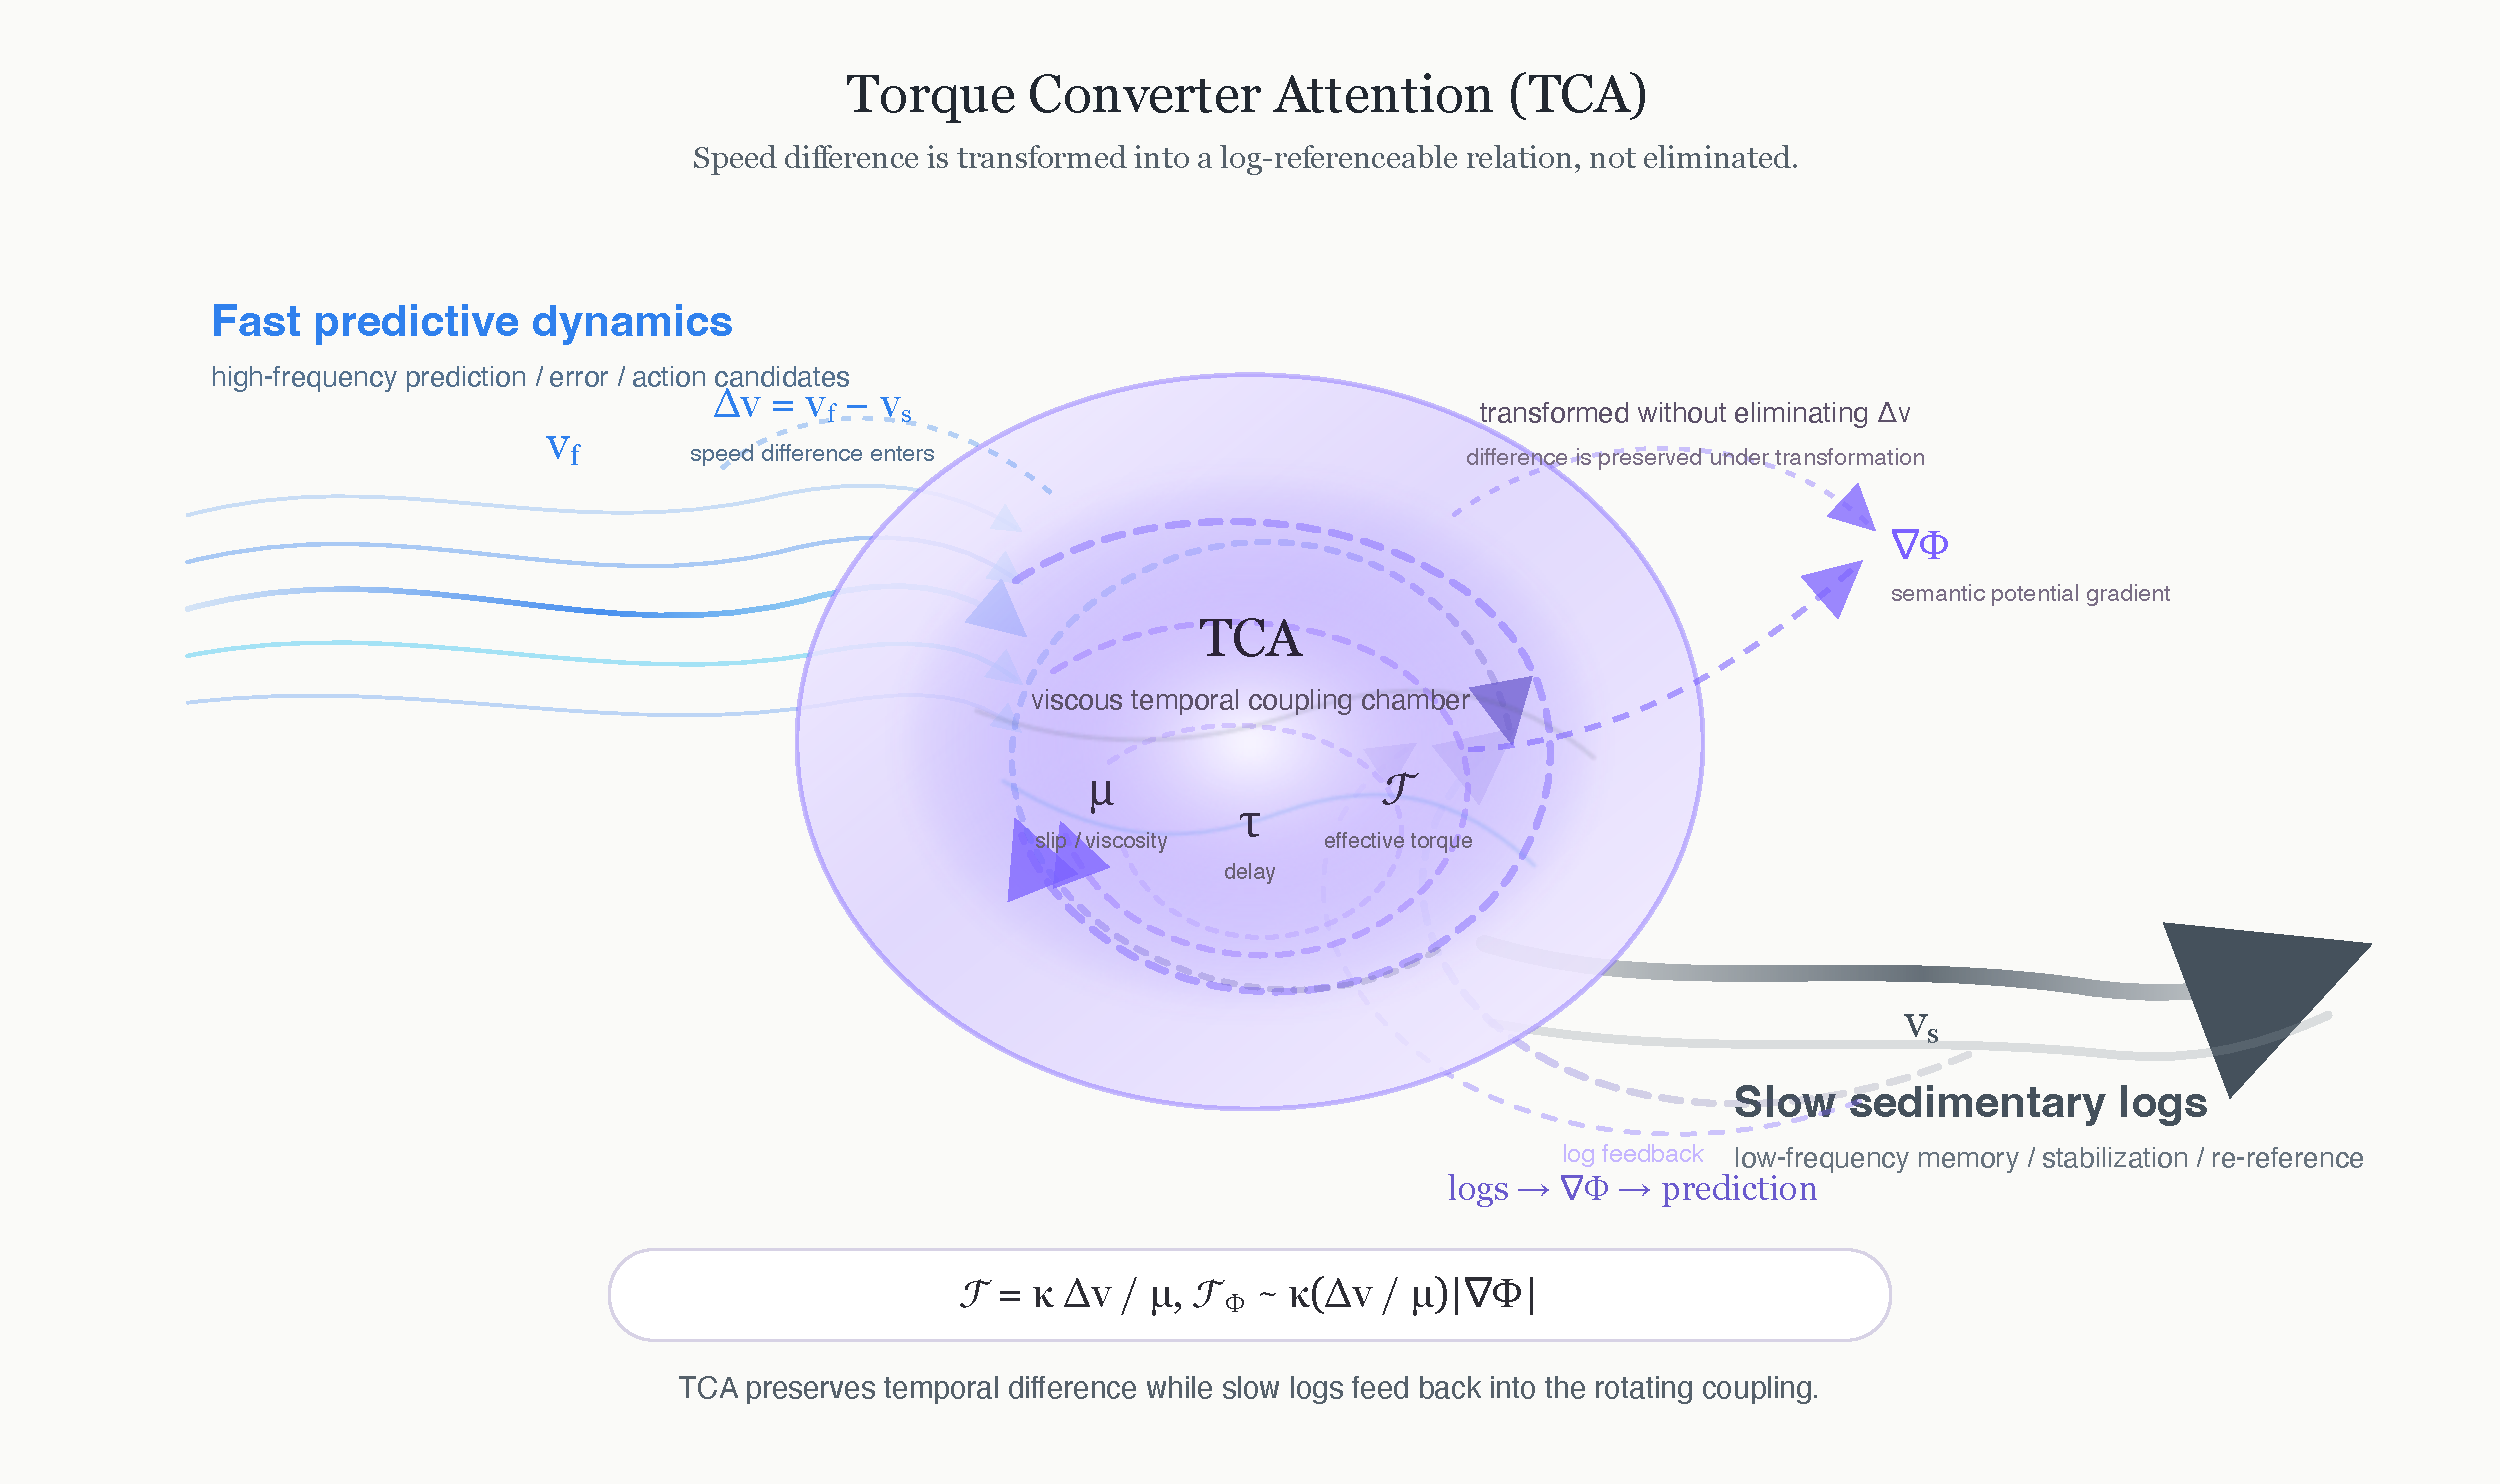
\includegraphics[width=0.92\linewidth]{figures/figure2_tca.pdf}
\caption{
Torque Converter Attention (TCA).
TCA preserves temporal difference while transforming it into a log-referenceable relation.
Fast predictive dynamics, slow sedimentary logs, coupling viscosity, delay, and effective torque are coupled without eliminating the speed difference.
}
\label{fig:tca}
\end{figure}

\subsection{Attention as Temporal Transformation}


From this perspective, Attention is not a selection mechanism but a temporal transformation mechanism.

Attention does not copy fast processing directly into slow processing.

Nor does slow processing control fast processing from above.

Attention transforms the predictions, expectations, errors, and reactions arising in the fast layer into a time window referenceable by the slow layer.

This transformation involves delay $\tau$:

\begin{equation}
\tau \propto \frac{\Delta v}{\mu}
\end{equation}

This delay is not mere processing lag.

It is the temporal thickness through which current processing sediments into past logs and becomes re-referenceable.

Attention therefore determines not "where to look" but "which speed difference, over which time window, with how much slip, is passed through."

In this sense, Attention is not a psychological term but a temporal control term.

\begin{quote}
\textbf{Correspondence with CT (Conceptual Topography §4.2):} In Conceptual Topography, linguistic tokens $\ell_i$ couple locally to $\nabla\Phi$ and deepen potential wells through repeated use. The coupling term
\[
\lambda \sum_i \ell_i \cdot \nabla\Phi
\]
corresponds to the TCA operation of "transforming speed difference along the meaning gradient." TCA is a transformation mechanism along the temporal axis; CT's token coupling is a transformation mechanism along the spatial axis. The two can be read as different cross-sections of the same transformation structure.
\end{quote}

\subsection{From Attention to Ego}


This paper holds that Torque Converter Attention corresponds to the position experienced as the ego.

However, the ego referred to here is not a subject.

The ego is not a judge, a command center, or a decision-maker.

The ego is the dynamic position at which the speed difference between the fast and slow layers concentrates and is transformed.

Humans tend to experience this transformation point as the place where they are thinking, the place where they are choosing, the place where they are conscious.

But this does not mean that the ego is the cause of action.

Rather, the ego is the point where action preparation, memory sedimentation, and log referencing intersect.

The ego is therefore not an illusion.

It has a clear function.

But equally, the ego is not a subject.

It is the transformation point required when dual plasticity and temporal asymmetry are established.

\subsection{Relation to Log Referencing}


Torque Converter Attention is important because it makes log referencing possible.

Processing arising in the fast layer disappears as it is.

Logs sedimented in the slow layer are not connected to the present as they are.

When Torque Converter Attention operates between the two, a referencing relation opens between current processing and past logs.

At this point, fast-layer processing is not fully absorbed into the slow layer.

Slow-layer logs do not fully dominate the fast layer.

The two couple while retaining their speed difference.

This non-closed coupling is the precondition for consciousness as a log-referencing state.

\subsection{Bridge to IFGT and VED}


The discussion so far has defined Torque Converter Attention as a problem of speed difference and coupling viscosity.

However, in a conscious state, which logs are easily referenced is not determined by speed difference alone.

Log referencing is directed by the meaning gradient.

The next section therefore introduces information density $I$, information flow $J_I$, local log-referencing flow $J_{\log}$, and information potential $\Phi$, and maps this torque-like quantity onto the structure of IFGT and VED.

There, the effective torque-like quantity $\mathcal{T}$ is extended to $\mathcal{T}_{\Phi}$, which includes the meaning gradient:

\begin{equation}
\mathcal{T}_{\Phi} \sim \kappa \frac{\Delta v}{\mu} |\nabla \Phi|
\end{equation}

This expression does not generate consciousness.

It is a structural index showing, when speed difference, coupling viscosity, and meaning gradient simultaneously obtain, in which direction and with what strength log referencing tends to open.

Torque Converter Attention is therefore not merely an analogy in this paper.

It is a VED-type mechanism that transmits speed difference while preserving non-closure, and an IFGT-type mechanism that directs log referencing along the meaning gradient.
